\begin{center}{ \bf  Невыпуклые топологические биллиарды как модели интегрируемых геодезических потоков на ориентируемых поверхностях}\\
{\it А.Т.Фоменко } \\
(Москва; {\it atfomenko@mail.ru} )\\
{\it В.В.Ведюшкина } \\
(Москва; {\it arinir@yandex.ru} )

\end{center}
\addcontentsline{toc}{section}{Фоменко А.Т., Ведюшкина В.В.}


Две интегрируемые системы называются лиувиллево эквивалентными, если существует диффеоморфизм, переводящий
слоение Лиувилля одной системы в слоение Лиувилля другой системы. Если
торы Лиувилля на всюду плотном множестве являются замыканиями нерезонансных траекторий (как в большинстве невырожденных  классических случаев интегрируемости), то лиувиллева эквивалентность систем означает, что сравниваемые системы имеют ``одинаковые'' замыкания решений (т.е. интегральных траекторий) на трёхмерных уровнях постоянной энергии.   Топологический тип слоения Лиувилля
полностью определяется инвариантом Фоменко--Цишанга, который является
некоторым графом с числовыми метками (см. подробнее книгу Болсинова А.В., Фоменко А.Т. [1], и работу Фоменко А.Т., Цишанга Х. [2]).

 Пусть дана замкнутая компактная  двумерная поверхность. Рассмотрим геодезический поток на ней. Оказывается, такой геодезический поток в аналитическом случае является интегрируемым в том только случае когда поверхность гомеоморфна сфере, тору, проективной плоскости или бутылке Клейна (Козлов В.В. [3]).

 Далее, для линейно и квадратично  интегрируемых геодезических потоков   были вычислены   инварианты Фоменко-Цишанга (см. работы [4-6]). Оказалось, что схожие инварианты возникают для других интегрируемых систем -- топологических биллиардов.


Пусть  область $\Omega$  на плоскости $\mathbb{R}^2$  такова, что граница области является кусочно-гладкой кривой, причём в точках излома этой кривой углы равны $\frac{\pi}{2}$.
Рассмотрим биллиард, описывающий движение (материальной) точки внутри области $\Omega$ с
естественным отражением на границе $P=\partial \Omega$.    Будем считать, что в точках,
где граница $P$ не гладкая
(тогда, как было сказано,  угол излома обязательно равен $\frac{\pi}{2}$)
 траектории системы можно доопределить по непрерывности: а именно, попав в вершину угла границы, материальная точка, не теряя скорости, отразится назад по той же траектории.
 Фиксируем декартовы координаты $(x,y)$ на плоскости $\mathbb{R}^2.$ Рассмотрим семейство софокусных квадрик -- кривых,  задаваемых соотношением

$$ (b-\lambda)x^2+(a-\lambda)y^2=(a-\lambda)(b-\lambda),   \lambda\leqslant a.$$


Как заметили В.В.Козлов и Д.В.Трещёв (см. [7]) касательные в любой точке биллиардной траектории внутри области $\Omega,$ ограниченной дугами софокусных квадрик,
касаются эллипса или гиперболы, софокусных с семейством квадрик, образующих границу $P$ биллиарда $\Omega$.
Относительно стандартной симплектической структуры на плоскости, функции $|v|^2$ --- квадрат модуля вектора скорости -- и $\Lambda$ --- параметр софокусной квадрики
коммутируют. Так как они сохраняются вдоль траекторий биллиарда, значит в пределе они коммутируют и на границе биллиардной области.
 Таким
образом, данная   система имеет два независимых   интеграла  --   квадрат модуля вектора скорости (или энергия) и параметр софокусной квадрики, обозначаемый через $\Lambda.$
Рассмотрим следующие топологические биллиарды, полученные склейкой из плоских биллиардов вдоль сегментов границ (обозначения и описание областей см. [8]): $\Delta_\alpha(2(A_1+nA_0+2mB_1+4mnB_0+A_1)) $ (гомеоморфен сфере)
и
  $\Delta_{\alpha eh}(2n \widetilde{B_0}) $ (гомеоморфен тору), а  также следующий топологический биллиард с четырьмя коническими точками $\Delta_{\beta eh}(2n \widetilde{B_0})  $ (см. рис.~\ref{topologicalbilliards}). Оказывается, при выборе подходящих областей слоение Лиувилля соответствующих изоэнергетической поверхности описывается той же молекулой, что и квадратично интегрируемый геодезический поток   сферы (для биллиардов, гомеоморфных сфере) и тора (для биллиардов, склеенных из $B_0$) с глобально лиувиллевой метрикой или линейно интегрируемым геодезическим потоком.  Таким образом удалось установить лиувиллеву эквивалентность    интегрируемых геодезических потоков на ориентируемых поверхностях топологическим  биллиардам  с помощью сравнения меченых молекул. Тем самым, образно говоря, топологические  интегрируемые биллиарды ``наглядно моделируют''  все линейно и квадратично интегрируемые геодезические потоки на двумерных  ориентируемых поверхностях. Напомним, что аналитический геодезический поток на двумерной ориентируемой замкнутой поверхности интегрируем в том и только в том случае, когда поверхность гомеоморфна сфере или тору.  При этом, хорошо известно описание римановых метрик, геодезические потоки которых допускают линейные или квадратичные по импульсам интегралы. См. подробный обзор, например, в [1].





  \begin{figure}[h!]

  \center{ 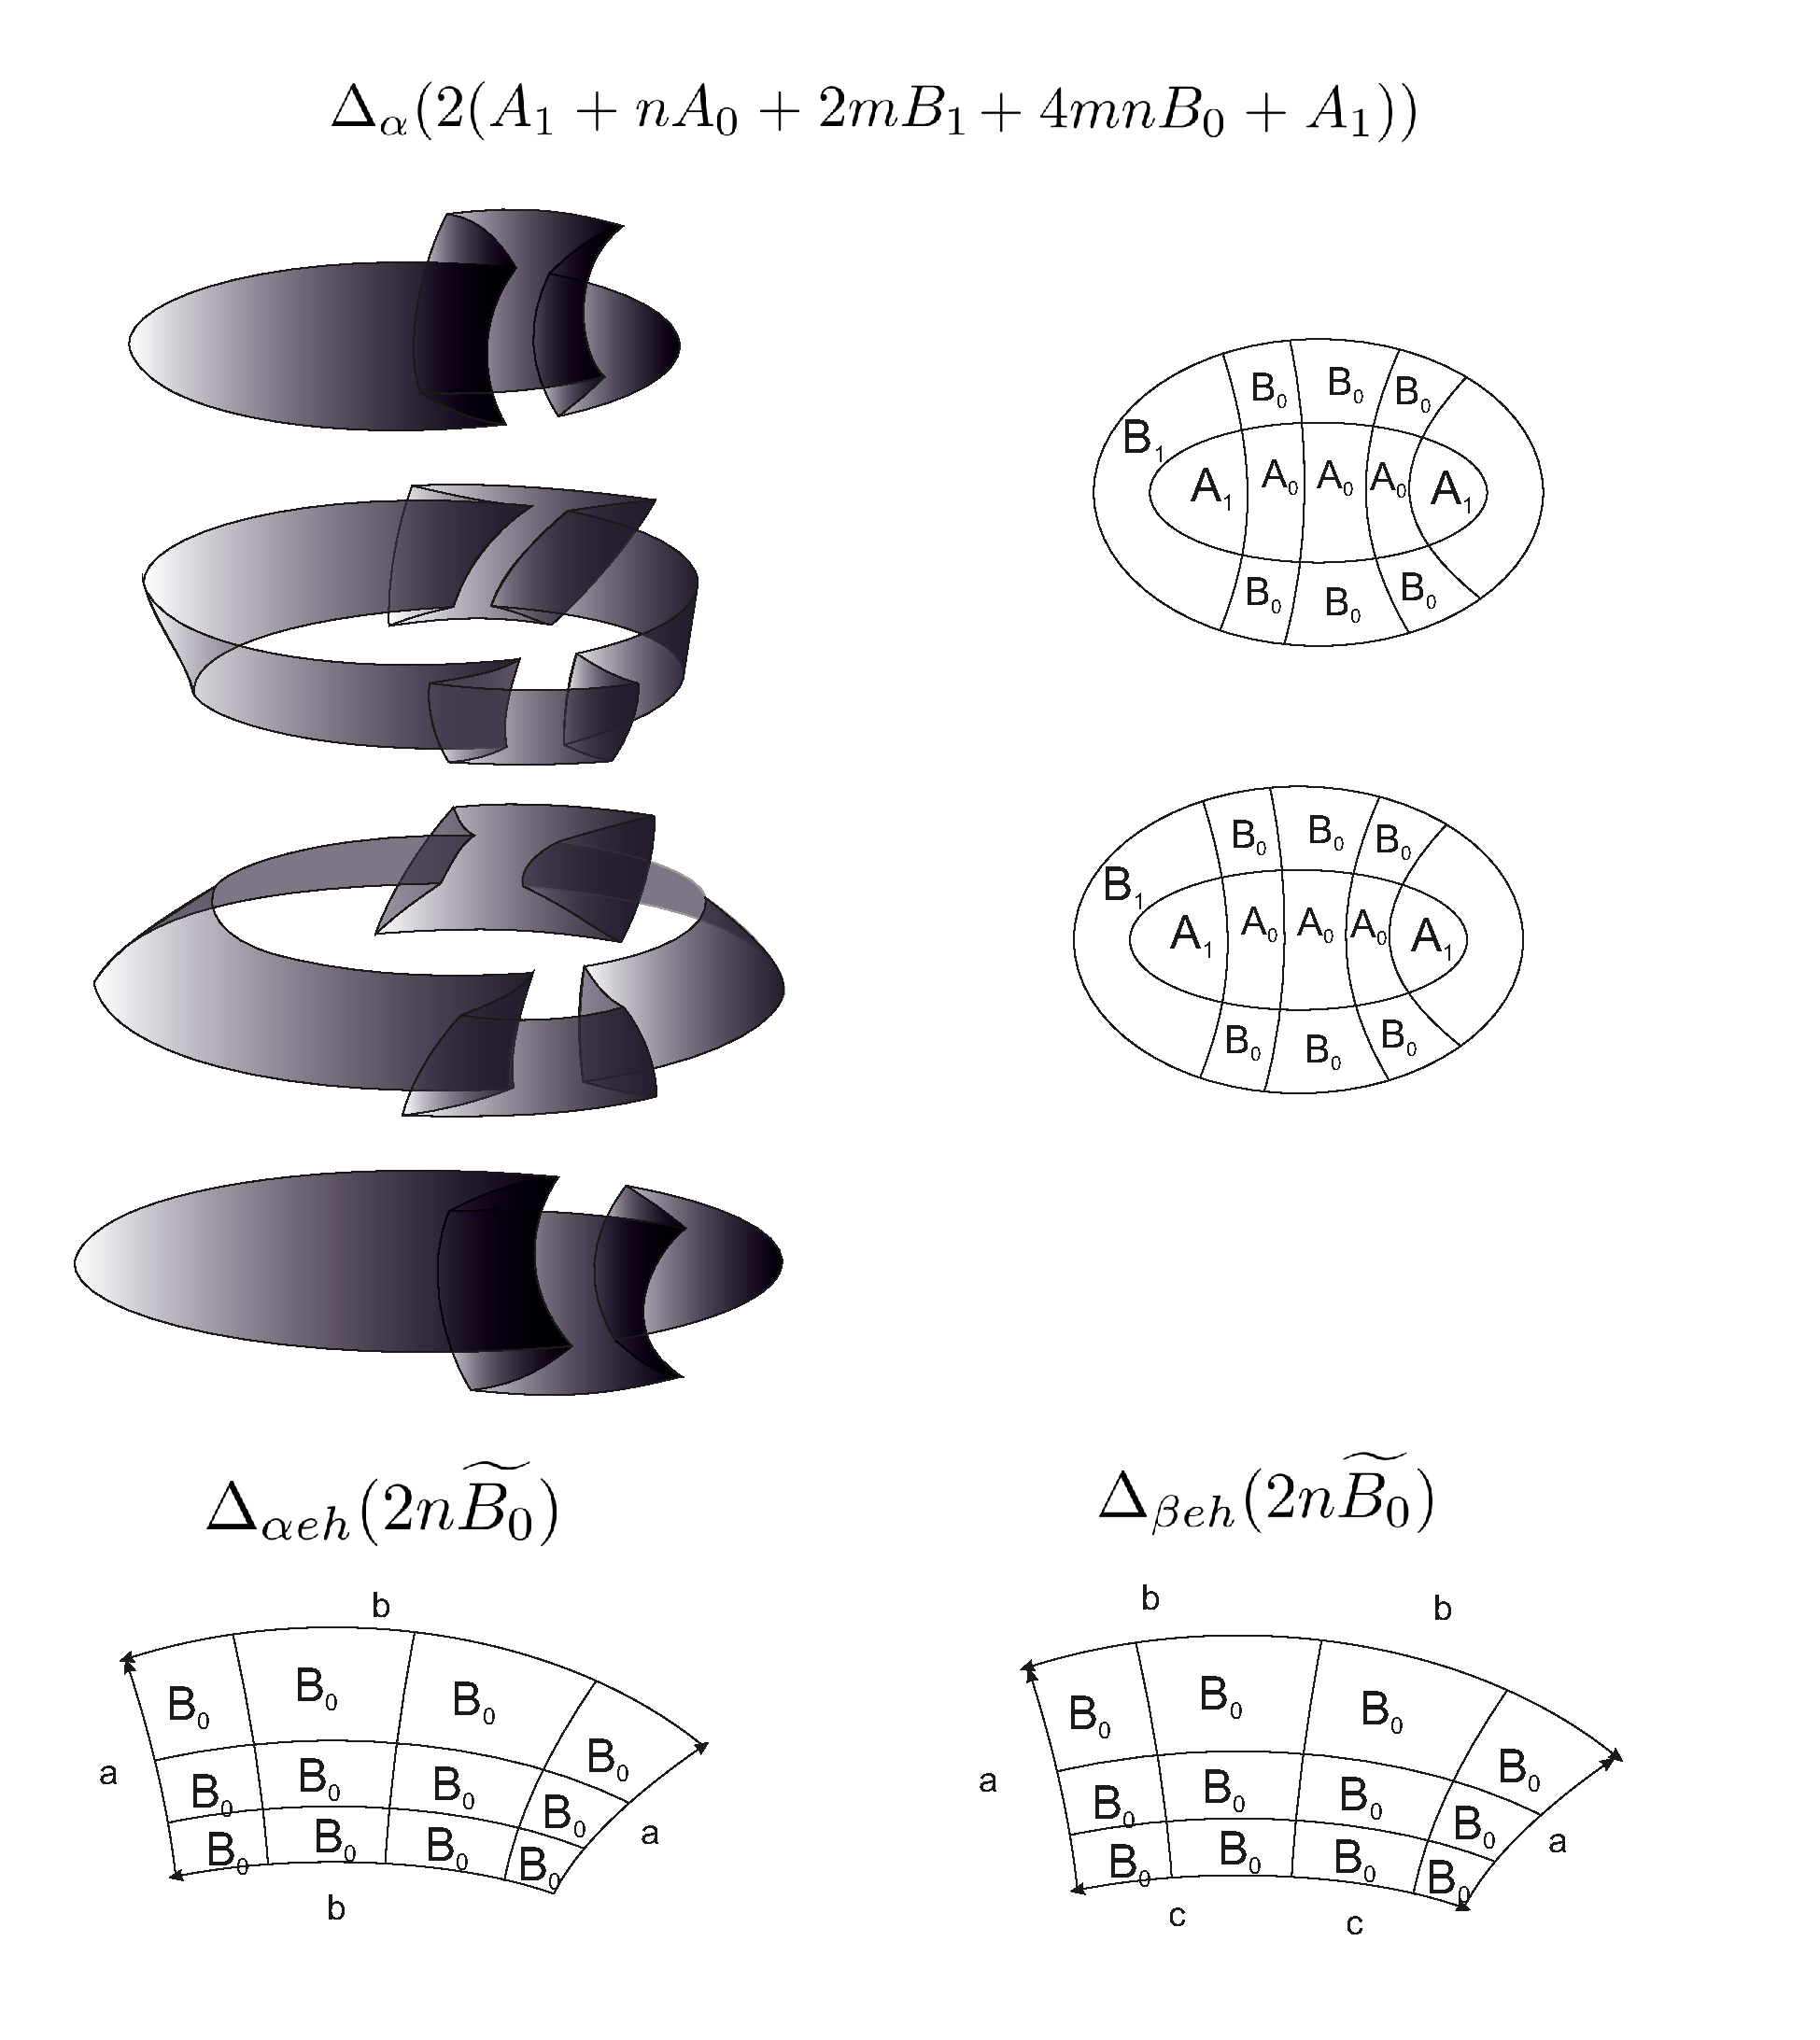
\includegraphics[width=\textwidth]{Fomenko_Vedushkina_topologicalbilliards.pdf}}

  \caption{Топологические биллиарды:  $\Delta_\alpha(2(A_1+nA_0+2mB_1+4mnB_0+A_1))  $ и $\Delta_{\beta eh}(2n \widetilde{B_0})  $ (гомеоморфные сфере)
и
  $\Delta_{\alpha eh}(2n \widetilde{B_0}) $ (гомеоморфен тору). }\label{topologicalbilliards}
\end{figure}

\textbf{Теорема.}{\it

а) Квадратично-интегрируемый геодезический поток двумерной сферы на  изоэнергетической трёхмерной поверхности лиувиллево эквивалентен топологическому двумерному интегрируемому биллиарду   $\Delta_\alpha(2(A_1+nA_0+2mB_1+4mnB_0+A_1))   $ (см. рис.~\ref{topologicalbilliards}).

б) Геодезический поток двумерного тора с глобально лиувиллевой метрикой (то есть допускающий квадратичный интеграл) на изоэнергетической трёхмерной поверхности лиувиллево эквивалентен топологическому двумерному интегрируемому биллиарду $\Delta_{\alpha eh}(2n \widetilde{B_0})  $ (см. рис.~\ref{topologicalbilliards}).

в) Геодезический линейно-интегрируемый поток двумерного тора на трёхмерной изоэнергетической поверхности лиувиллево эквивалентен топологическому двумерному интегрируемому биллиарду  $\Delta_{\beta eh}(2n \widetilde{B_0})   $ (см. рис.~\ref{topologicalbilliards}).
}


\smallskip \centerline{\bf Литература}\nopagebreak



1. {\it Болсинов А.В, Фоменко А.Т.} Интегрируемые гамильтоновы системы.
Геометрия, топология, классификация, Т.1,2,
   Ижевск
   НИЦ ``Регулярная и хаотическая динамика'',
  1999
2. {\it  Фоменко А.Т., Цишанг Х.} О типичных топологических свойствах
интегрируемых гамильтоновых систем,  Изв. АН СССР
   52:2(1988),
  378--407

  3.{\it Козлов В.В. } Топологические препятствия к интегрируемости натуральных механических систем, ДАН СССР, 249:6 (1979), 1299-1302

  4. {\it Селиванова Е.Н. }Классификация геодезических потоков лиувиллевых метрик на двумерном торе с точностью до топологической эквивалентности,  Матем. сб., 183:4 (1992), 69-86

   5. {\it Матвеев В.С. } Особенности отображения момента и топологическое строение интегрируемых геодезических потоков. Диссертация на осискание учёной степени к.ф.-м.н.,  Москва, МГУ, мех-матем. ф-т, 1996

    6. {\it Нгуен Т.З., Полякова Л.С., Селиванова Е.Н.} Топологическая классификация интегрируемых геодезических потоков с дополнительным квадратичным или линейным по импульсам интегралом на двумерных ориентируемых римановых многообразиях, Функциональный анализ, 27:3 (1993), 42-56

  7. {\it Козлов В.В., Трещёв Д.В.} Генетическое  введение в динамику систем с ударами. М.: Изд-во МГУ, 1991

  8. {\it Ведюшкина В.В.} Слоение Лиувилля невыпуклых топологических биллиардов, ДАН, 478:1(2018)
